\documentclass{beamer}

\mode<presentation>
{
  \usetheme{Frankfurt}
  \usecolortheme{orchid}
  \setbeamercovered{invisible}
  \setbeamertemplate{footline}[frame number]
}

\usepackage[english]{babel}
\usepackage[latin1]{inputenc}
\usepackage{times}
\usepackage[T1]{fontenc}
\usepackage{tikz}
\usepackage{array}
\usepackage{cancel}


\usetikzlibrary{shapes,backgrounds}

\def\multiset#1#2{\ensuremath{\left(\kern-.3em\left(\genfrac{}{}{0pt}{}{#1}{#2}\right)\kern-.3em\right)}}

\def\blue{\color{blue}~}
\def\black{\color{black}~}
\def\bl[#1]#2{\begin{block}{#1}#2\end{block}}
\def\integers{\mathbb{Z}}
\def\enumb{\begin{enumerate}}
\def\enume{\end{enumerate}}
\def\itemb{\begin{itemize}}
\def\iteme{\end{itemize}}


\usepackage{remreset}
\makeatletter
\@removefromreset{subsection}{section}
\makeatother
\setcounter{subsection}{1}

\title{Discrete Mathematics, Section 002, Spring 2016}
\subtitle{Lecture 9: Multisets, Inclusion-Exclusion formula}

\author[Zsolt]{Zsolt Pajor-Gyulai \\ \texttt{zsolt@cims.nyu.edu}}

\pgfdeclareimage[height=1cm]{NYUlogo}{NYUlogo.jpg}

\institute[NYU] 
{
\normalsize Courant Institute of Mathematical Sciences
}
\titlegraphic{\pgfuseimage{NYUlogo}}

\begin{document}

\begin{frame}
  \titlepage
\end{frame}

\AtBeginSection[]
{
\begin{frame}
\frametitle{Outline}
\tableofcontents[currentsection]
\end{frame}}

\section{Multisets}
\begin{frame}{Fundamental counting problems}
So far we have studied three counting problems:

\begin{figure}
\centering
\begin{tabular}{|c|c|c|}
\hline
&With repetition&Without repetition\\
\hline
\textbf{Ordered}&$n^k$&$(n)_k$\\
\hline
\textbf{Unordered}&$?$&$\binom{n}{k}$\\
\hline
\end{tabular}
\end{figure}
\[
n:\textrm{ Size of universe},\qquad k: \textrm{ Size of collection}
\]
Now we fill in the gap.
\end{frame}

\begin{frame}{Multisets}
\vspace{-0.2cm}

\bl[Multiset]{
An unordered collection of elements where an element can be included more than once.
}
For example: 
\[
\langle 1,2,3,3\rangle,\quad \langle 1, 5, 5, 7, 7, 9, 9\rangle
\]
These are still unordered collections and therefore
\[
\langle 1,2,3,3\rangle=\langle 3,2,1, 3\rangle=\langle 2, 3, 3, 1\rangle
\]\vspace{-0.6cm}
\itemb
\item \textbf{Multiplicity:} The multiplicity of an element is the number of time it is a member of the multiset.
For example the multiplicity of $3$ in $\langle 1,2,3,3\rangle$ is two.
\item \textbf{Cardinality:} The cardinality of a multiset is the sum of multiplicities of its elements.
\iteme
\end{frame}

\begin{frame}{Counting multisets}
\bl[`n multichoose k']{
Let $n,k\in\mathbb{N}$. The symbol $\multiset{n}{k}$ denotes the number of multisets with cardinality equal to $k$ whose elements belong to an $n$-element set such as $\{1,2,\dots,n\}$.
}

\begin{figure}
\centering
\begin{tabular}{|c|c|c|}
\hline
&With repetition&Without repetition\\
\hline
\textbf{Ordered}&$n^k$&$(n)_k$\\
\hline
\textbf{Unordered}&$\multiset{n}{k}$&$\binom{n}{k}$\\
\hline
\end{tabular}
\end{figure}
\[
n:\textrm{ Size of universe},\qquad k: \textrm{ Size of collection}
\]
\end{frame}

\begin{frame}{Examples}
\enumb
\item Do the two examples directly on your worksheet!
\item One element multisets are
\[
\langle 1\rangle,\dots,\langle n\rangle
\]\vspace{-0.7cm}

Therefore $\multiset{n}{1}=n$.
\item There is only one $k$-element multiset with elements selected from $\{1\}$, namely
\[
\langle\underbrace{1,\dots,1}_{k}\rangle,
\]\vspace{-0.8cm}

and so $\multiset{1}{k}=1$.
\item If $n=2$, then we have to select the multiplicity of $1$, and then the remaining places get filled with $2$-s. Therefore
\[
\multiset{2}{k}=k+1
\]
\item For special values, do Problem 2 on the Worksheet.
\enume

\end{frame}

\begin{frame}{`Pascal's triangle' for multisets}
\begin{figure}
\centering
\begin{tabular}{|c|ccccccc|}
\hline
k&0&1&2&3&4&5&6\\
\hline
$n=0$&1&0&0&0&0&0&0\\
$n=1$&1&1&1&1&1&1&1\\
$n=2$&1&2&3&4&5&6&7\\
$n=3$&1&3&6&10&15&21&28\\
$n=4$&1&4&10&20&35&56&84\\
$n=5$&1&5&15&35&70&126&210\\
$n=6$&1&6&21&56&126&252&462\\
\hline
\end{tabular}
\end{figure}

\bl[Proposition]{
\[
\multiset{n}{k}=\multiset{n-1}{k}+\multiset{n}{k-1}
\]
}

For the proof see the textbook (p103).
\end{frame}

\begin{frame}{Formula for $\multiset{n}{k}$}
\bl[Proposition]{
\[
\multiset{n}{k}=\binom{n+k-1}{k}
\]
}
Idea of the proof for $n\geq 1$:
\itemb
\item Order the elements in the multiset in increasing order.
\[
\langle 1,1,1,2,3,3,5\rangle\qquad\textrm{out of }\{1,2,3,4,5,6\}
\]
\item Put bars when a new element is used
\[
\langle 1,1,1|,2|,3,3||,5|\rangle
\]
\item Replace the elements by stars
\[
***|*|**||*|
\]
\iteme
\end{frame}

\begin{frame}{Formula for $\multiset{n}{k}$}
\bl[Proposition]{
\[
\multiset{n}{k}=\binom{n+k-1}{k}
\]
}
Idea of the proof for $n\geq 1$:
\itemb
\item We can do this the other way around, take e.g.
\[
***|||*||***|*||
\]
\item This translates into
\[
\langle 1,1,1,4,6,6,6,7\rangle
\]
\item The original set can be also read off to be 
\[
\{1,2,3,4,5,6,7,8,9\}
\]
\iteme
Do this yourself on Problem 3 on the worksheet!
\end{frame}

\begin{frame}{Formula for $\multiset{n}{k}$}
\bl[Proposition]{
\[
\multiset{n}{k}=\binom{n+k-1}{k}
\]
}
Idea of the proof for $n\geq 1$:
\itemb
\item For a general $n$ and $k$ there are $k$ stars and $n-1$ bars.
\item We need to choose the $k$ places where to put the stars, then the rest of the places will be occupied by the bars.
\iteme
For a formalized proof, see the textbook.
\end{frame}

\section{Inclusion-Exclusion}

\begin{frame}{Inclusion-exclusion formula for two sets}
\bl[]{\center{$|A\cup B|=|A|+|B|-|A\cap B|$}}

For example: How many integers in the range $1$ to $1000$ (inclusive) are divisible by $2$ or by $5$?\pause
\[
A=\{x\in\mathbb{Z}: 1\leq x\leq 1000\textrm{ and }2|x\}
\]
\[
B=\{x\in\mathbb{Z}: 1\leq x\leq 1000\textrm{ and }5|x\}
\]\pause
Then $|A|=500$ and $|B|=200$. Also note
\[
A\cap B=\{x\in\mathbb{Z}: 1\leq x\leq 1000\textrm{ and }10|x\}
\]
and therefore $|A\cap B|=100$.\pause Therefore
\[
|A\cup B|=|A|+|B|-|A\cap B|=500+200-100=600.
\]\pause
Therefore there are $600$ integers in the range $1$ to $1000$ that are divisible by either $2$ or $5$.
\end{frame}

\begin{frame}{Inclusion-exclusion formula for three sets}
\bl[]{\vspace{-0.5cm}
\[
|A\cup B\cup C|=\uncover<1->{|A|+|B|+|C|}\uncover<2->{-|A\cap B|-|A\cap C|-|B\cap C|}\uncover<3->{+|A\cap B\cap C|.}
\]\vspace{-0.6cm}}
\begin{figure}
\centering
\begin{tikzpicture}[scale=1.5]
\draw (2,2) circle (1cm);
\draw (3,2) circle (1cm);
\draw (2.5,1) circle (1cm);

\only<1>{
\node at (1.5,2.25) {$1$};
\node at (3.5,2.25) {$1$};
\node at (2.5,0.5) {$1$};

\node at (1.9,1.3){$2$};
\node at (3.1,1.3){$2$};
\node at (2.5,2.3){$2$};

\node at (2.5,1.6){$3$};
}

\only<2>{
\node at (1.5,2.25) {$1$};
\node at (3.5,2.25) {$1$};
\node at (2.5,0.5) {$1$};

\node at (1.9,1.3){$1$};
\node at (3.1,1.3){$1$};
\node at (2.5,2.3){$1$};

\node at (2.5,1.6){$0$};
}

\only<3>{
\node at (1.5,2.25) {$1$};
\node at (3.5,2.25) {$1$};
\node at (2.5,0.5) {$1$};

\node at (1.9,1.3){$1$};
\node at (3.1,1.3){$1$};
\node at (2.5,2.3){$1$};

\node at (2.5,1.6){$1$};
}
\end{tikzpicture}
\caption{Number of times elements in each `compartment' are counted.}
\end{figure}
\end{frame}

\begin{frame}{Inclusion-exclusion formula for three sets}
\bl[]{\vspace{-0.5cm}
\[
|A\cup B\cup C|=|A|+|B|+|C|-|A\cap B|-|A\cap C|-|B\cap C|+|A\cap B\cap C|.
\]}
At an art academy, there are 43 students taking ceramics, 57 students taking painting, and 29 students taking sculpture. There are 10 students in both ceramics and painting, 5 in both painting and sculpture, 5 in both ceramics and sculpture, and 2 taking all three courses. How many students are taking at least one course at the art academy?
\[
|C\cup P\cup S|=|C|+|P|+|S|-|C\cap P|-|C\cap S|-|P\cap S|+|C\cap P\cap S|=
\]
\[
=43+57+29-10-5-5+2=111
\]
\end{frame}

\begin{frame}{Inclusion-exclusion formula for more sets}
\bl[Four sets]{\vspace{-0.5cm}
\begin{align*}
|A&\cup B\cup C\cup D|=|A|+|B|+|C|+|D|-\\
&-|A\cap B|-|A\cap C|-|A\cap D|-|B\cap C|-|B\cap D|-|C\cap D|+\\
&+|A\cap B\cap D|+|A\cap B\cap D|+|A\cap C\cap D|+|B\cap C\cap D|-\\
&-|A\cap B\cap C\cap D|.
\end{align*}
}
Try this with Problem 4 on the worksheet!

\end{frame}

\begin{frame}{Inclusion-exclusion formula for more sets}

\bl[Theorem]{\vspace{-0.5cm}
\begin{align*}
|A_1&\dots\cup A_n|=|A|+\dots+|A_n|-\\
&-|A_1\cap A_2|-|A_1\cap A_3|-\dots-|A_{n-1}\cap A_n|+\\
&+|A_1\cap A_2\cap A_3|+\dots+|A_{n-2}\cap A_{n-1}\cap A_n|-\\
&-\dots+\dots\dots\\
&\pm|A_1\cap \dots \cap A_n|.
\end{align*}
}
For a proof, see the textbook.

\end{frame}



\end{document}